\section{What is Science?}

\begin{frame}
  \begin{center}
    Part I: First, What is Science?
  \end{center}
\end{frame}

\subsection{Definitions}
\begin{frame}{What is Science?}
  At the end of your 2-year course, you will receive a diploma that says:
  \begin{center}
    Master in Computer \structure{Science}
  \end{center}
  What do these words mean?
  \medskip
  
  Let's have some discussion about this (and let me learn about you too!)
  \bigskip

  \begin{block}<2>{Some answers from students in past years}
    \begin{itemize}
      \item Science is a method to learn about the world;
      \item Science is a method to reach the truth;
      \item Science is useful when it contributes to society;
      \item Science is how we develop new technologies;
    \end{itemize}
  \end{block}\bigskip
\end{frame}

\begin{frame}{Thinking about science}{(Not answering the question...)}
  \begin{itemize}
    \item "Science" can mean different things, for different people, depending on context... not very satisfying.
    \medskip

    \item But maybe there are some common threads in the discussion
    ("science", the word, meaning knowledge):
    \begin{itemize}
      \item The act of discovering knew knowledge about the world;
      \item An activity that requires precision, detail, curiosity and honesty;
      \item An activity that requires inspiration and creativity;
      \item Trying to improve society, trying to improve technology\\
      (are these the same? are other entities that ask for improvement?)
    \end{itemize}
    \item There are also some threads that are not often discussed:
    \begin{itemize}
      \item Science as a {\bf community}
      \item Science as a {\bf continuous process}
      \item The relationship between {\bf science and society} (is this relationship two way?)
    \end{itemize}
  \end{itemize}
\end{frame}

\begin{frame}{What is Science}{I know it when I see it}

  One way to understand science is to think about people, institutions, and events that we think of as "scientific", and reflect about them.\bigskip 

  \begin{block}{}
    I also think it is important for us to have many role models we can get inspiration from.\\
    It is good to have heroes!
  \end{block}
  \bigskip

  Let's talk a little about some famous scientists and scientific events.
\end{frame}

\subsection{Marie Curie}
\begin{frame}{Marie Curie}{Fact Sheet}
  \begin{columns}
    \column{.3\textwidth}
  \includegraphics[width=1\textwidth]{../img/irasutoya_curie}
  \ppagenote{Marie Curie sketch from \url{https://www.irasutoya.com}}\\
    \column{.7\textwidth}

    \begin{itemize}
      \item Marie Curie was Chemist from Poland. She discovered serveral radioactive materials and their properties.
      \medskip
      
      \item Won two nobel prizes: Physics and Chemistry\\
      (only person to receive two nobels in different scientific fields)
    \end{itemize}
  \end{columns}
\end{frame}

% Scientific Background
\begin{frame}{Marie Curie}{Scientific Background}
  \hfill\includegraphics[width=.25\textwidth]{../img/marie_pierre_curie}\ppagenote{Marie and Pierre Curie image from Wikipedia (Public Domain)}
  \begin{itemize}
    \item Why did some materials emit radiation?
    \begin{itemize}
      \item Was it a result of interaction between elements? Or a property of the element itself?
      \item One of Curie's early significant discoveries was that the quantity of radiation depends only on the amount of the material.
    \end{itemize}
    \item What is radiation useful for?
    \begin{itemize}
      \item Until then, radiation was a pretty curiosity.
      \item Curie developed several medical uses for radiation.
    \end{itemize}
  \end{itemize}
\end{frame}

\begin{frame}{Marie Curie}{Medical applications of radiation}
  \begin{itemize}
    \item Observed that cancer tumour cells died more quickly to radiation than healthy cells;
    \item Designed mobile X-ray equipment that could be used for surgery in World War I ("little curies");
    \item Designed Radon gas syringes for sterilizing tissue and wounds;
  \end{itemize}

  \hfill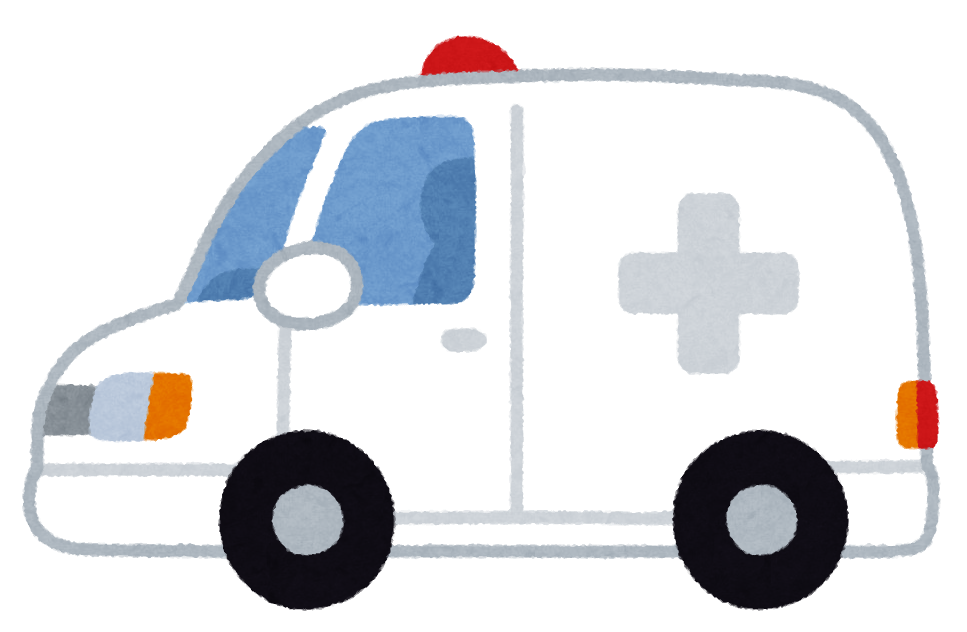
\includegraphics[width=0.3\textwidth]{../img/irasutoya_ambulance.png}
  \ppagenote{Ambulance from \url{https://www.irasutoya.com}}
\end{frame} 

\begin{frame}[t]{Marie Curie}{Open Science}
  \begin{itemize}
    \item Refused to patent Radium or the technologies to extract and develop the material;
    \item Result: a Radium boom spread across the world, increasing its usage and study;
    \item She believed that by sharing scientific discoveries, this would allow science (and society) to progress faster.
  \end{itemize}

  \vfill
  \begin{quote}
    "Physicists should always publish their researches completely. If our discovery has a commercial future that is a circumstance from which we should not profit. If radium is to be used in the treatment of disease, it is impossible for us to take advantage of that." 
  \end{quote}
  \hfill About the patenting of radium
\end{frame}

\begin{frame}{Marie Curie}{Personal Background}
  \begin{columns}
  \column{0.3\textwidth}
    \includegraphics[width=1\textwidth]{../img/marie_curie_sister}\ppagenote{Curie sisters image from Wikipedia (public domain)}
  \column{0.7\textwidth}
  \begin{itemize}
    \item Studied in an "underground university" (Flying University), and had to work as a tutor to support herself;\medskip
    
    \item Difficulty to get funding, sourcecrowded some of her research materials;\medskip
    
    \item Difficulties related to gender relations in Europe;\medskip

    \item The dangers of radioactivity were not well understood at the time: 
    \begin{itemize}
      \item Died early from radiation related diseases (like many chemists at the time);
      \item Her research notebooks are still radioactive today!
    \end{itemize}
  \end{itemize}
  \end{columns} 
\end{frame}

\begin{frame}{Marie Curie}{Legacy}

  What can we learn from the stories of famous scientists?\bigskip 

  What are the scientists and stories that you know, that inspire you?

\end{frame}

\subsection{Scientific Discoveries}


\begin{frame}[t]{What is Science?}{Scientific Discoveries}

  To define "science", it is also helpful to think about events that you consider as "scientific".\bigskip

  How are discoveries made?\bigskip

  Let's talk about two interesting discoveries.

\end{frame}

% CMB 
% -- research about radiation from the starts from 1890
% -- discovery by chance in 1965
% -- confirmation of the big bang theory

\begin{frame}{Example 1: The Origins of the Universe}{Discovery of the Cosmic Background Radiation and confirmation of the Big Bang Theory}

  \begin{columns}[T]

    \column{0.6\textwidth}
    \begin{itemize}
    \item The origins of the universe is a key topics in physics research. However, it is "not very easy" to find data about this ancient event;\bigskip 
    
    \item The Cosmic Background Radiation, a faint noise that can be detected everywhere, supports the theory that the universe was originally hot and dense, and expanded quickly;\bigskip 
    
    \item It was discovered in 1965 by chance, when two astronomers found a noise in their telescope that they could not remove in any way, no matter how;
    \end{itemize}
    \column{0.4\textwidth}
    \includegraphics[width=.9\textwidth]{../img/nasa_cmb}
    \ppagenote{1- CMB images from NASA (public domain)}
  \end{columns}
\end{frame}


\begin{frame}{Example 1: The Origins of the Universe}{Behind "chance" discoveries, there is a lot of preparation}

  \begin{columns}[T]

    \column{0.6\textwidth}
    Behind the "chance" discovery of CMB, there was a lot of preparation in reality.\medskip

    \begin{itemize}
      \item Scientists had investigated microwave radiation from the stars since 1890;\medskip
      
      \item A theoretical model for CMB had been predicted in 1948 by a different group;\medskip
      
      \item A third group was actively searching for the same data, and helped the chance findings;\medskip

    \end{itemize}
    \column{0.4\textwidth}
    \includegraphics[width=.7\textwidth]{../img/nasa_cmb_data}
    \ppagenote{2- CMB images from NASA (public domain)}
  \end{columns}\bigskip

  Luck smile on those who are prepared (including humanity as a whole!)
\end{frame}

%%%%%%%%%%%%%%%%%%%%%%%%%%%%%%%%%%%%%%%%%%%%%%%%%

\begin{frame}{Example 2: Proving that Citrus Fruit prevents Scurvy}{Hail Britannia!}
  
  In the 18th century, the British Empire needed a large navy to control and plunder its dominion around the world.\bigskip

  However, sailors who spent too much time at sea would suffer a terrible {\bf Rotting Disease}, which caused weakness, fatigue, bleeding, and eventually death from infection. This disease made constant stops at shore necessary.\bigskip

  Today we know that this disease, called {\bf scurvy} is caused by the \structure{lack of vitamin C}. But the way that the British Navy dealt with the problem is an interesting case of experimentation.
\end{frame}

% TODO: change CITRUS slide so it does not use a single huge image.
\begin{frame}{Example 2: Citrus fruits prevents scurvy}{James Lind's experiment}
  \begin{center}
    \includegraphics[height=.8\textheight]{../img/wikipedia_scurvy}
    \ppagenote{James Lind image from Wikipedia, Public Domain}
  \end{center}
\end{frame}

\begin{frame}{Example 2: Proving that Citrus Fruit prevents Scurvy}{Aftermatch}
  Of course, before Lind's experiment, there was already folk knowledge and recommendation about the relationship of Scurvy and Citrus. This includes memoirs by Spanish, French and Portuguese explorers.\bigskip

  Nevertheless, Lind's experiment is interesting to consider as an example of a general idea being formally demonstrated through a controlled experiment!\bigskip 

  In spite of this experiment, the British Navy only formally started adding Lemon Juice to its rations from 1790...
\end{frame}

% \item Understanding Science \url{https://undsci.berkeley.edu/article/intro_01}

\begin{frame}{A Framework for Science}{}
  Thinking about scientists and scientific discoveries, we start to see science as "something" with a set of characteristics. But what is it?\bigskip

  Many of you might have learned the following description in high school or university:

  \begin{block}{The Scientific Method}
    \begin{enumerate}
      \item Observe a Phenomenom
      \item Propose a Hypothesis
      \item Perform an Experiment
      \item Draw conclusions
    \end{enumerate}
  \end{block}\bigskip

  Is this a good description of "What is Science?"
\end{frame}

\begin{frame}{"The Scientific Method" -- Too simple!}{}
  \begin{columns}
    \column{0.6\textwidth}
      This description of the scientific method has a kernel of truth. But it has some limitations when compared to how science is actually done:
    \column{0.4\textwidth}
      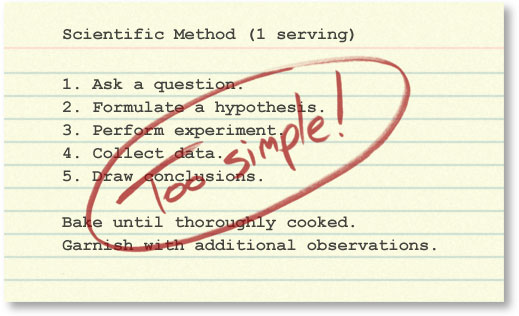
\includegraphics[width=1\textwidth]{../img/scientific_method_simple}
      \ppagenote{"Too simple" image: University of California Museum of Paleontology's Understanding Science}
  \end{columns}
  \vfill

  {\smaller
  \begin{itemize}
    \item It does not explain where questions or hypothesis come from.
    \item What happens when two scientists disagree about the data?
    \item It assumes that the scientific process ends after the data is collected.\\
      \hfill (How does this new knowledge reach society?)\\
      \hfill (How does this new knowledge influence science?)
    \item It assumes that old hypothesis or data never gets reviewed.
    \item etc...
  \end{itemize}
  }
\end{frame}

\begin{frame}{Science as an Interactive Process}{}
  A more complete view of the process of science involves ideas, data, the scientific community, and society, in a continuous feedback circle.
  \begin{center}
    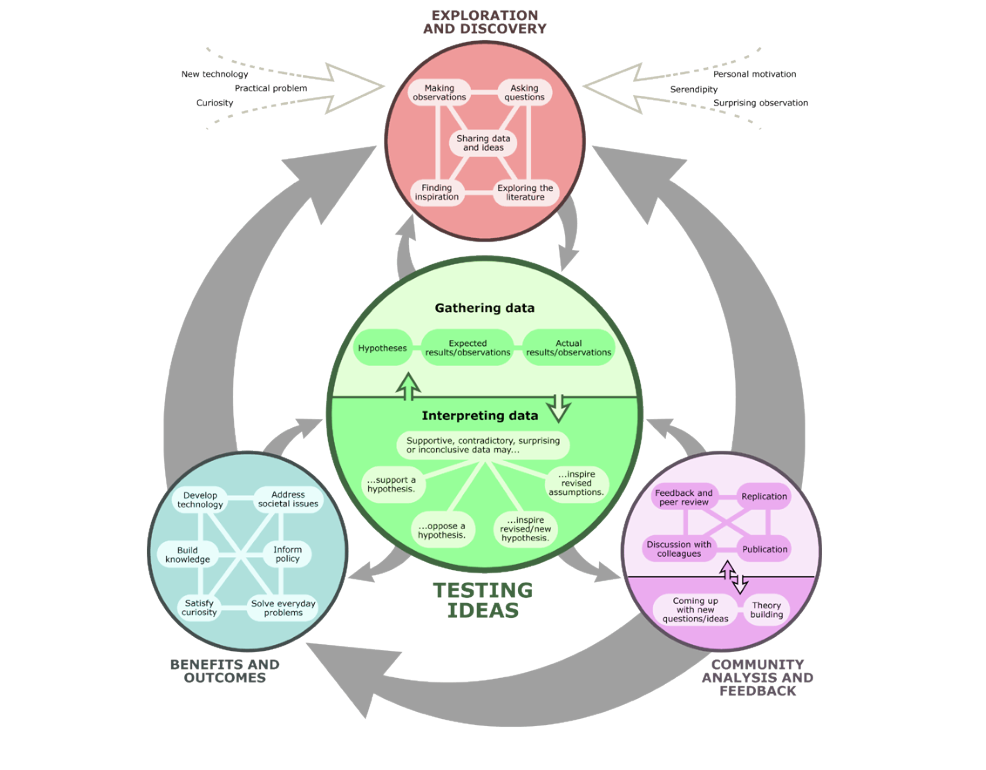
\includegraphics[width=0.5\textwidth]{../img/understandingscience_realprocess1}\ppagenote{"Real Process of Science 1" image: University of California Museum of Paleontology's Understanding Science}
  \end{center}
\end{frame}

\begin{frame}{Science as an Interactive Process}{}
  This understanding helps us see that there are many different paths to scientific discoveries. And these paths still have some common characteristics tying them together.
  \begin{center}
    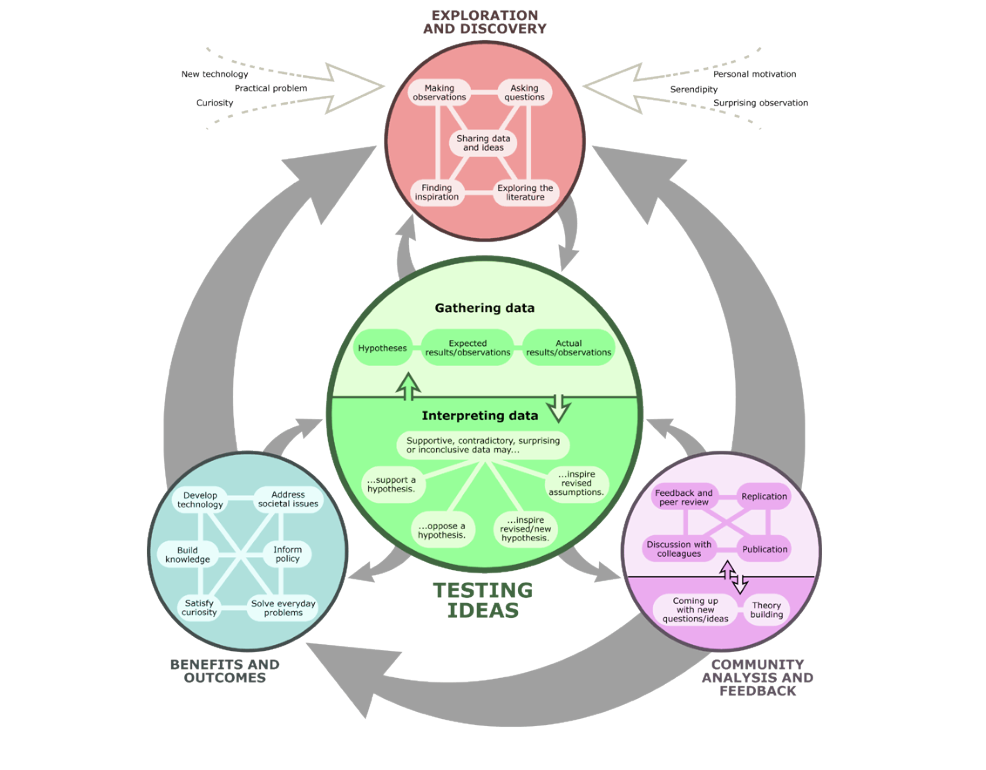
\includegraphics[width=0.5\textwidth]{../img/understandingscience_realprocess1}
    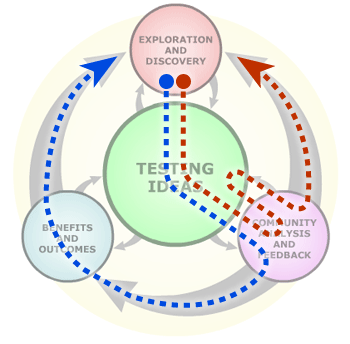
\includegraphics[width=0.4\textwidth]{../img/understandingscience_realprocess2}\ppagenote{"Real Process of Science 2" image: University of California Museum of Paleontology's Understanding Science}
  \end{center}
\end{frame}

\begin{frame}{Science as an Interactive Process -- Breakdown}{Where do ideas come from?}
  \begin{center}
    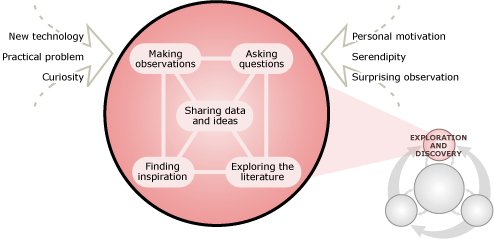
\includegraphics[width=0.8\textwidth]{../img/understandingscience_zoom1}\ppagenote{"Real Process of Science Zoom 1" image: University of California Museum of Paleontology's Understanding Science}
  \end{center}
\end{frame}

\begin{frame}{Science as an Interactive Process -- Breakdown}{Testing and Experimentation}
  \begin{center}
    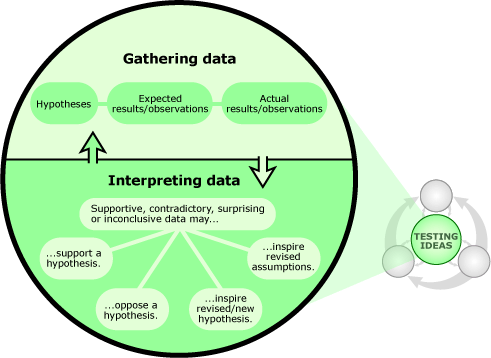
\includegraphics[width=0.6\textwidth]{../img/understandingscience_zoom2}\ppagenote{"Real Process of Science Zoom 2" image: University of California Museum of Paleontology's Understanding Science}
  \end{center}
\end{frame}

\begin{frame}{Science as an Interactive Process -- Breakdown}{The Scientific Community}
  \begin{center}
    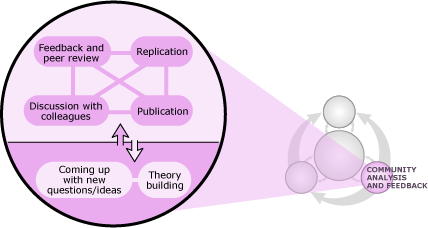
\includegraphics[width=0.8\textwidth]{../img/understandingscience_zoom3}\ppagenote{"Real Process of Science Zoom 3" image: University of California Museum of Paleontology's Understanding Science}
  \end{center}
\end{frame}

\begin{frame}{Science as an Interactive Process -- Breakdown}{Science and Society}
  \begin{center}
    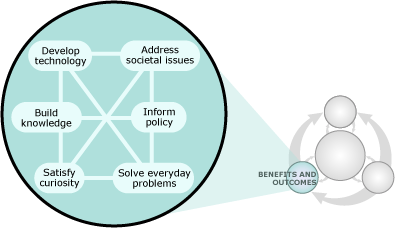
\includegraphics[width=0.7\textwidth]{../img/understandingscience_zoom4}\ppagenote{"Real Process of Science Zoom 4" image: University of California Museum of Paleontology's Understanding Science}
  \end{center}
\end{frame}

\subsection{Wrap-up}
\begin{frame}{Wrap up -- What is Science?}
  \begin{itemize}
    \item Science is a method, a way of thinking, and also a community. A process of search and discovery that is continuously changing our society.
    \item I highly recommend that you read the \structure{"Understanding Science"} webpage, for a much more in-depth discussion. See the manaba links.
    \item {\bf What about Computer Sciences}? Popular discussion of science usually focus on physics, biology, social science, etc. How does Computer Science fit in this framework?
    \vfill

    \item In the next part of the lecture, we are going to focus on the role of experiments in science, which is also the focus for the rest of this class.
  \end{itemize}
\end{frame}
